\subsection{LDView}\label{podsekce-ldview}
\begin{figure}[htbp]
        \centering
        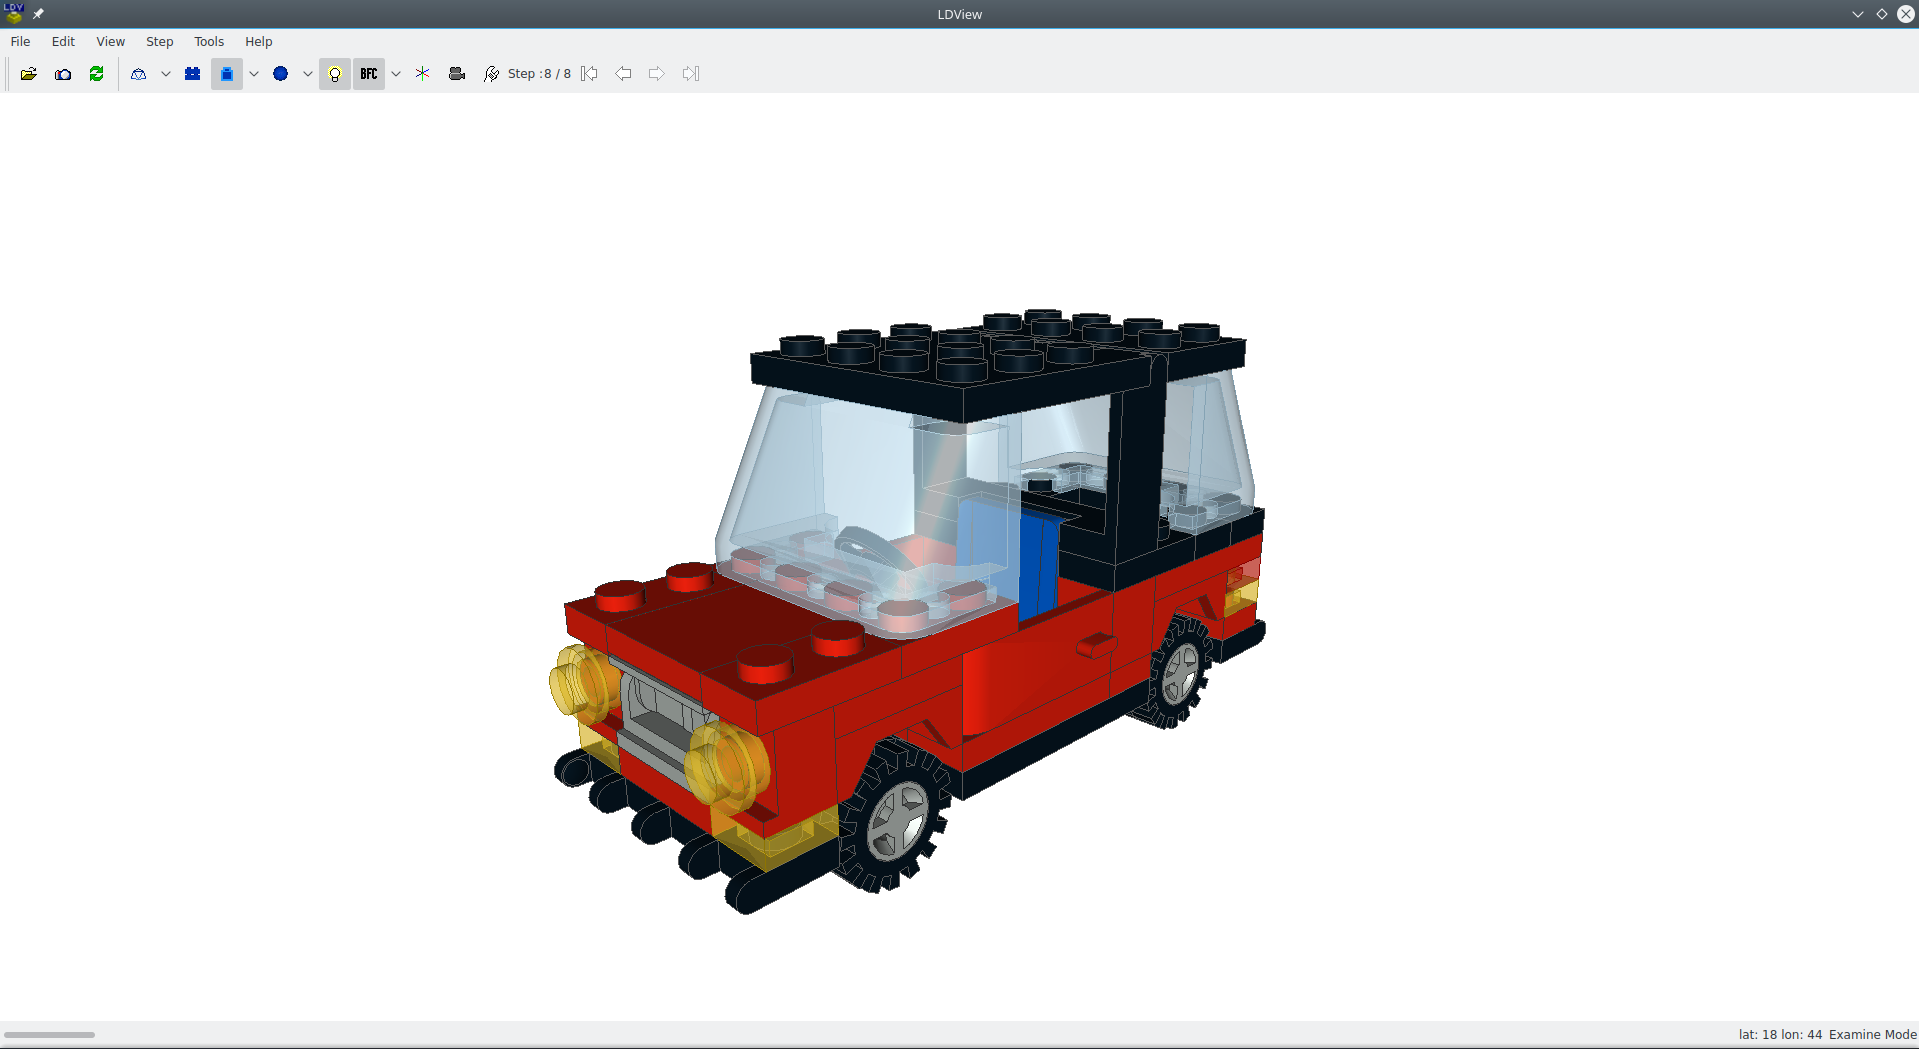
\includegraphics[width=\textwidth,height=\textheight,keepaspectratio]{images/ldview.png}
        \caption{Snímek obrazovky programu LDView}
\end{figure}

LDView je 3D prohlížeč modelů a součástek ve formátu LDraw, představeného v~sekci \emph{\nameref{ldraw-format}} na straně \emph{\pageref{ldraw-format}}. Program je veřejně dostupný pod licencí \gls{GPLv2} \autocite{GPLv2}.

Mezi jedny z~funkcí programu patří: 
\begin{itemize}
    \item schopnost exportovat LDraw modely do formátů \textit{POV-Ray}, \textit{3DS} nebo \textit{STL},
    \item schopnost pořizovat snímek aktuálního pohledu.
\end{itemize}

Program je dostupný jak ve verzi s~grafickým prostředím, tak v~konzolové verzi využitelné například na systémech bez grafického prostředí.

Pro více informací o~programu a jeho dostupných funkcích doporučuji \autocite{ldview}.

\subsubsection*{Převod formátu}

Převod formátu LDraw do jiných formátů pomocí programu LDView je velmi jednoduchý. V~ukázce \emph{\ref{priklad-ldview}} je příklad použití konzolové verze programu. 

Při konzultaci s~vedoucím bylo odhaleno, že převedené součástky mají 10krát menší meřítko a jsou o~90° otočené kolem osy X. Formát \textit{\gls{STL}} dle specifikace \autocite{stl:specification} nemá jednotku a není definováno, která osa ukazuje směrem vzhůru. Při \gls{FDM} 3D tisku je však praxí, že se předpokládá jenotka mm a osa Z~směřující vzhůru. Z~tohoto důvodu je vhodné provést korekci souborů \textit{STL}.

Oprava těchto chyb ve zdrojovém kódu programu by stála velké množství práce a náročné zorientování se v~cizím kódu. Proto jsem se rozhodl opravu měřítka a natočení modelu provést pomocí nástroje ADMesh. 

 \begin{listing}[htbp]
        \begin{minted}{bash}
$ ldview ./ldraw/parts/3003.dat -LDrawDir=./ldraw -ExportFile=3003.stl 
        \end{minted}
    \caption{Příklad použití programu LDView \label{priklad-ldview}}
\end{listing}


